\documentclass[xcolor=table]{beamer}

\usepackage{bm}

\usepackage{movie15}
\usepackage{xcolor}
\usepackage{graphicx}
\usepackage{outlines}
\usepackage[cal=cm]{mathalfa}
\DeclareMathOperator*{\argmin}{arg\,min}
\DeclareMathOperator*{\argmax}{arg\,max}
\DeclareMathOperator{\tr}{tr}
\usepackage[table]{xcolor}

\graphicspath{{figures/}}

\newcommand{\hlw}[1]{{\color{blue!80!black} #1}}


%TITLE PAGE
\title{\bf \huge Bayesian Regression on Inverse Dynamics of SARCOS arm}
\author{\Large Teguh Santoso Lembono}
\date{\it Bayesian Computation - \today}

\setbeamersize{text margin left=6pt,text margin right=10pt}
\setbeamertemplate{itemize items}[circle]
\setbeamertemplate{frametitle}{\vspace{2mm}\bfseries
\insertframetitle}
\setbeamertemplate{sidebar right}{}
\setbeamertemplate{footline}{%
\hfill\usebeamertemplate***{navigation symbols}
\hspace{1cm}\insertframenumber{}/\inserttotalframenumber}



%STARTING DOCUMENT
\begin{document}
\maketitle


%PAGE 1
\begin{frame}

\frametitle{Problem Definition: Inverse Dynamics}

\centering

\begin{itemize}
\item SARCOS arm is a 7 Degree-of-Freedoms (DoFs) robot

\item Given the current joint positions, velocities, and accelerations, the inverse dynamics problem is to predict the torques at each joint. 

\item Input $\bm{x}:(\bm{\theta}, \dot{\bm{\theta}}, \ddot{\bm{\theta}}) \in \mathbb{R}^{21}$, output $\bm{\tau} \in \mathbb{R}^{7}$ 

\item In this presentation, I only consider the first torque, $\tau_1$

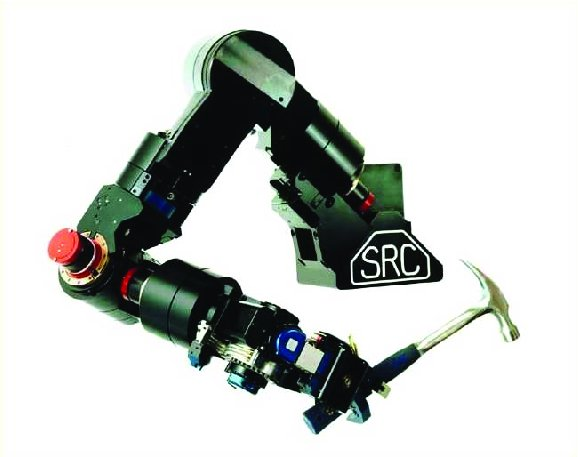
\includegraphics[height=0.4\columnwidth]{SARCOS_arm}

\end{itemize}

\end{frame}



%PAGE 3
\begin{frame}
\frametitle{Methods Overview}
\begin{outline}
\1 Linear Regression with GVA
\1 Linear Regression with Laplace Approximation
\1 Linear Regression with Polynomial Input Feature and Laplace Approximation
\1 Gaussian Mixture Regression with Bayesian EM
\end{outline}
\end{frame}


%PAGE 2
\begin{frame}
\frametitle{Validation Method}
\centering

\begin{itemize}
\item Standardized Mean Squared Error (sMSE)
\begin{equation}
MSE = \frac{1}{N}\sum_i^N(y_i - f(\bm{x}_i))^2
\end{equation}

\begin{equation}
sMSE = \frac{MSE}{var(\bm{y})}
\end{equation}

\item Mean Standardized Log Loss (MSLL)
\begin{equation}
LL_i = \frac{1}{2}\log(2\pi\sigma_i^2) + \frac{(y_i - f(\bm{x}_i))^2}{2\sigma_i^2}
\end{equation}
\begin{equation}
SLL_i = LL_i - LL_{i,mean}
\end{equation}
\begin{equation}
MSLL = \frac{1}{N}\sum_i^N(SLL_i)
\end{equation}

\item $y_i$ and $f(\bm{x}_i)$ are the true and prediction value, respectively
\end{itemize}
\end{frame}


\begin{frame}
\frametitle{Linear Regression with GVA}
\begin{itemize}

\item The likelihood is formulated as a linear model:
\begin{equation}
p(y|\bm{x},\bm{w},\lambda) = \mathcal{N}\left(\bm{w}^\top \bm{x}, \lambda^{-1}\mathbcal{I}\right)
\end{equation}
\item The prior of $\bm{w}$ and $\lambda$ is Gaussian and Gamma distribution, respectively
\begin{equation}
p(\bm{w}) = \mathcal{N}\left(\bm{0}, \alpha\mathbcal{I}\right)
\end{equation}
\begin{equation}
p(\lambda) = \textit{Gamma}\left(a,b\right)
\end{equation}

\item The posterior is computed by minimizing the negative ELBO

\end{itemize}
\end{frame}

\begin{frame}
\frametitle{Linear Regression with Laplace Approximation}
\centering
\begin{itemize}
\item The likelihood and the prior are the same as the first method
\item The posterior is computed by doing Laplace Approximation:
\begin{equation}
p(\bm{w}|\bm{X},\bm{Y}) = \mathcal{N}\left(\bm{w}_{MAP}, Hess(\bm{w}_{MAP})^{-1}\right)  
\end{equation}
\end{itemize}
\end{frame}

\begin{frame}
\frametitle{Linear Regression with Polynomial Input Features and Laplace Approximation}
\centering
\begin{itemize}

\item Similar to the previous method, but the input is modified by second order polynomial mapping
\begin{equation}
(x) \rightarrow (1, x, x^2)
\end{equation}
\begin{equation}
(x_1, x_2) \rightarrow (1, x_1, x_2, x_1x_2, x_1^2, x_2^2 )
\end{equation}
%
for all input dimension

\item The input dimension increases from 21 to 253

\item The posterior is computed by Laplace Approximation
\end{itemize}

\end{frame}

\begin{frame}
\frametitle{Gaussian Mixture Regression}
\centering
\begin{itemize}
\item Gaussian Mixture Regression (GMR) is used a lot in robot learning
\item Given the input $\bm{x}$ and the output $y$, the joint distribution is formulated as Gaussian Mixture Model: 
\begin{equation}
p(\bm{x},y) = \sum_k^K \pi_k \mathcal{N}(\bm{\mu_k},\bm{\Sigma_k})
\end{equation}
\item Given a new input $\bm{x}^*$, the predictive distribution is computed by conditioning on $\bm{x}^*$. The method is commonly referred to as GMR
\begin{equation}
p(\bm{y}|~\bm{x}^*,\bm{\theta}) = \sum_k^K p(k|~\bm{x}^*,\bm{\theta}) p(\bm{y}|~k,\bm{x}^*,\bm{\theta}), 
\end{equation}
where $\bm{\theta}$ is the set of GMM parameters, 
\begin{equation}
\bm{\theta} = \{\bm{Z}, \pi_k,\bm{\mu}_k, \bm{\Sigma}_k |~k \in [0, K-1]\}
\end{equation}
\end{itemize}

\end{frame}

\begin{frame}
\frametitle{Gaussian Mixture Regression with Bayesian EM}
\centering
\begin{itemize}
\item Here the posterior distribution of $\bm{\theta}$ is computed using Variational Inference with Factorized Distribution
\item The following priors are assigned to $\bm{\theta}$:
\begin{equation}
p(\bm{\pi}) = \textit{Dirichlet}(\bm{\alpha})
\end{equation}
\begin{equation}
p(\bm{\mu}) = \mathcal{N}\left(0, \beta^{-1} \mathbcal{I}\right)
\end{equation}
\begin{equation}
p(\bm{\Sigma}) = \textit{InvWishart}(\bm{\mathcal{W}}_0,v)
\end{equation}

\item The posterior distribution of $\bm{\theta}$ is approximated as a factorized distribution:
\begin{equation}
q(\bm{Z}, \bm{\pi},\bm{\mu}, \bm{\Sigma}) = q(\bm{Z})q(\bm{\pi},\bm{\mu}, \bm{\Sigma})
\end{equation}


\item The posterior can then be computed using steps similar to Expectation-Maximization, iterating between computing $q(\bm{Z})$ and $q(\bm{\pi},\bm{\mu}, \bm{\Sigma})$
\end{itemize}
\end{frame}

\begin{frame}
\frametitle{Comparison Result: sMSE}
\centering

\renewcommand{\arraystretch}{1.3}
\begin{table}[t]
\centering
\caption{sMSE result for different methods}
\begin{tabular}{l c c}
\hline
$\textbf{Method}$ & $\textbf{Training}$ & $\textbf{Test}$ \\ \hline 
LR with GVA     	& 0.0741	& 0.0747	  \\
LR with LA      & 0.0741 	& 0.0747 	  \\
PolyLR with LA    	& 0.0351	& 0.0343	  \\
GMR with Factorized GVA &   0.0386	& 0.0383 \\
GPR &   -	& 0.011 \\
\hline
\end{tabular}
\label{tab:cartesian}
\end{table}



\end{frame}



\begin{frame}
\frametitle{Comparison Result: MSLL}
\centering
\renewcommand{\arraystretch}{1.3}
\begin{table}[t]
\centering
\caption{MSLL result for different methods}
\begin{tabular}{l c c}
\hline
$\textbf{Method}$ & $\textbf{Training}$ & $\textbf{Test}$ \\ \hline 
LR with GVA     	& -1.301	& -1.291	  \\
LR with LA      & -1.301	& -1.291	  \\
PolyLR with LA    	& -1.673	&-1.678	  \\
GMR with Factorized GVA & -1.73	& -1.73 \\
GPR &   -	& -2.15 \\
\hline
\end{tabular}
\label{tab:cartesian}
\end{table}

\end{frame}

\begin{frame}
\frametitle{Conclusion}
\begin{itemize}
\item Laplace Approximation is faster than GVA, but gives quite a good approximation
\item Using polynomial expansion of the inputs result in better matching of the data, but the number of input features increases exponentially with the degree of polynomials
\item Using multiple linear models (GMR) result in better matching of the data
\end{itemize}
\centering
\end{frame}


%PAGE 2
\begin{frame}
\frametitle{Thank you!}
\centering
\end{frame}





\end{document}